\documentclass[]{article}
\usepackage[letterpaper]{geometry}
\usepackage{mtsummit2015}
\usepackage{times}
\usepackage{url}
\usepackage{latexsym}
\usepackage{natbib}
\usepackage{layout}
\usepackage{graphicx}
\usepackage{color}
\usepackage{booktabs}

\newcommand{\confname}{MT Summit 2015}
\newcommand{\website}{\protect\url{http://www.amtaweb.org/}}
\newcommand{\contactname}{research track co-chair Yaser Al-Onaizan}
\newcommand{\contactemail}{onaizan@us.ibm.com} 
\newcommand{\conffilename}{mtsummit2015}
\newcommand{\downloadsite}{\protect\url{http://www.amtaweb.org/}}
\newcommand{\paperlength}{$12$ (twelve)}
\newcommand{\shortpaperlength}{$6$ (six)}
\newcommand\newcite{\citet}	% to get "Author (Year)" with natbib    

%% do not add any other page- or text-size instruction here

\parskip=0.00in

\begin{document}

% \mtsummitHeader{x}{x}{xxx-xxx}{2015}{45-character paper description goes here}{Author(s) initials and last name go here}
\title{\bf OpenNMT: Open-Source Toolkit for Neural Machine Translation}  

\author{\name{\bf Guillaume Klein} \hfill \addr{SYSTRAN}
\AND
        \name{\bf Yoon Kim} \hfill \addr{Harvard University}
\AND
       \name{\bf Yuntian Deng} \hfill \addr{Harvard University}
        \AND
       \name{\bf Jean Senellart} \hfill \addr{SYSTRAN}
        \AND
       \name{\bf Alexander M. Rush} \hfill \addr{Harvard University}
}

\maketitle
\pagestyle{empty}

\begin{abstract}
  We describe an open-source toolkit for neural machine translation
  (NMT).  The toolkit prioritizes efficiency, modularity, and
  extensibility with the goal of supporting NMT research into model
  architectures, feature representations, and source modalities, while
  maintaining competitive performance and reasonable training
  requirements. The toolkit consists of modeling and translation support,
  as well as detailed pedagogical documentation about the underlying
  techniques.
\end{abstract}

\section{Introduction}


Neural machine translation (NMT) is a new methodology for machine
translation that has led to remarkable improvements, particularly in
terms of human evaluation, compared to rule-based
and statistical machine translation (SMT) systems
\citep{wu2016google,systran}. Originally developed using pure
sequence-to-sequence models \citep{sutskever14sequence,Cho2014} and
improved upon using attention-based variants \citep{Bahdanau2015,Luong2015}, NMT has now become a widely-applied technique for machine
translation, as well as an effective approach for other related NLP
tasks such as dialogue, parsing, and summarization.

As NMT approaches are standardized, it becomes more important for the
machine translation and NLP community to develop open implementations
for researchers to benchmark against, learn from, and extend
upon. Just as the SMT community benefited greatly from toolkits like
Moses \citep{koehn2007moses} for phrase-based SMT and CDec
\citep{dyer2010cdec} for syntax-based SMT, NMT toolkits can provide a
foundation to build upon. A toolkit should aim to provide
a shared framework for developing and comparing open-source systems,
while at the same time being efficient and accurate enough to be used
in production contexts.


\begin{figure}
  \centering
  \includegraphics[width=\linewidth]{simple-attn}
  \label{fig:rnn}
  \caption{\small Schematic view of neural machine translation. The \textcolor{red}{red} source words are first mapped to word vectors and then fed into a recurrent neural network (RNN). Upon seeing the $\langle$eos$\rangle$ symbol, the final time step initializes a target \textcolor{blue}{blue} RNN. At each target time step, \textit{attention} is applied over the source RNN and combined with the current hidden state to produce a prediction $p(w_t| w_{1: t-1}, x)$ of the next word. This prediction is then fed back into the target RNN.}
\end{figure}

% In this work we describe a new open-source toolkit for developing
% neural machine translation systems, known as \textit{OpenNMT}. The
% system is motivated by frameworks, such as Moses and CDec developed
% for statistical machine translation (SMT). These toolkits aim to
% provide a shared frameworks for developing and comparing open-source
% SMT systems that are complete and flexible enough for research
% development, while at the same time being efficient and accurate
% enough to be used production contexts. 

Currently there are several existing NMT implementations. Many systems
such as those developed in industry by Google, Microsoft, and Baidu, are unlikely to be released with unrestricted
licenses. Many other systems such as \textit{GroundHog},
\textit{Blocks}, \textit{tensorflow-seq2seq}, \textit{tensorflow-nmt}, \textit{Tensor2Tensor}, \textit{Sockeye}, \textit{Neural Monkey}, \textit{lamtram}, and
our own \textit{seq2seq-attn}, exist mostly as research code. These
libraries provide important functionality but minimal support to
production users. On the other hand, there exist production systems such as \textit{Marian} that are efficient for production but unamenable for research purposes. Perhaps most promising is the University of
Edinburgh's \textit{Nematus} system originally based on NYU's NMT
system. Nematus provides high-accuracy translation, many options,
clear documentation, and has been used in several successful research
projects. In the development of this project, we aimed to build upon
the strengths of this system, while providing additional documentation
and functionality to provide a useful open-source NMT framework for
the NLP community in academia and industry.

With these goals in mind, we introduce \textit{OpenNMT}
(\url{http://opennmt.net}), an open-source toolikit for neural machine translation. Since its launch in December 2016, OpenNMT has become a collection of implementations targeting both academia and industry. The systems are designed to be simple to use and easy to extend, while maintaining efficiency and state-of-the-art accuracy. In
addition to providing code for the core translation tasks, OpenNMT was
designed with two aims: (a) prioritize training and test
efficiency, (b) maintain model modularity and readability hence research extensibility.

This engineering report describes how the system targets these
criteria. We begin by briefly surveying the background for NMT,
describing the high-level implementation details, and then describing
specific case studies for the two criteria.  We end by showing
benchmarks of the system in terms of accuracy, speed, and memory usage
for several translation and translation-like tasks.



\section{Background}

NMT has now been extensively described in many
excellent tutorials (see for instance
\url{https://sites.google.com/site/acl16nmt/home}). We give only
a condensed overview. 

NMT takes a conditional language modeling view of translation by modeling the
probability of a target sentence $w_{1:T}$ given a source sentence
$x_{1:S}$ as
$p(w_{1:T}| x) = \prod_{1}^T p(w_t| w_{1:t-1}, x; \theta)$. This
distribution is estimated using an attention-based encoder-decoder
architecture \citep{Bahdanau2015}. A source encoder recurrent neural
network (RNN) maps each source word to a word vector, and processes
these to a sequence of hidden vectors
$\mathbf{h}_1, \ldots, \mathbf{h}_S$.  The target decoder combines an
RNN hidden representation of previously generated words
($w_1, ... w_{t-1}$) with source hidden vectors to predict scores for
each possible next word. A softmax layer is then used to produce a
next-word distribution $ p(w_t| w_{1:t-1}, x; \theta)$. The source
hidden vectors influence the distribution through an attention pooling
layer that weights each source word relative to its expected
contribution to the target prediction. The complete model is trained
end-to-end to minimize the negative log-likelihood of the training
corpus. An unfolded network diagram is shown in Figure~\ref{fig:rnn}.


In practice, there are also many other important aspects that improve
the effectiveness of the base model. Here we briefly mention four
areas: (a) It is important to use a gated RNN such as an LSTM
\citep{hochreiter1997long} or GRU \citep{chung2014empirical} which help
the model learn long-term features. (b) Translation requires
relatively large, stacked RNNs, which consist of several vertical
layers (2-16) of RNNs at each time step \citep{sutskever14sequence}. (c)
Input feeding, where the previous attention vector is fed back into
the input as well as the predicted word, has been shown to be quite
helpful for machine translation \citep{Luong2015}.  (d) Test-time
decoding is done through \textit{beam search} where multiple
hypothesis target predictions are considered at each time
step. Implementing these correctly can be difficult, which motivates
their inclusion in an NMT framework.





% \begin{itemize}
% \item One column describing the technical details
% \end{itemize}
\begin{figure}
  \centering
  \includegraphics[width=\linewidth]{demo}
  \label{fig:live}
  \caption{\small Live demo of the OpenNMT system across dozens of language pairs.}
\end{figure}
\section{Implementation}

OpenNMT is a complete library for training and deploying neural
machine translation models. The system is successor to
\textit{seq2seq-attn} developed at Harvard, and has been completely
rewritten for ease of efficiency, readability, and
generalizability. It includes vanilla NMT models along with support
for attention, gating, stacking, input feeding, regularization, beam
search and all other options necessary for state-of-the-art
performance.  

OpenNMT has currently three main implementations with the same API suiting different needs, and all of them are actively maintained:

\paragraph{OpenNMT-lua} The original project developed with LuaTorch.
    Full-featured, optimized, and stable code ready for quick experiments and production.
\paragraph{OpenNMT-py} An OpenNMT-lua clone using the more modern PyTorch.
    Initially created by by Adam
Lerer and the Facebook AI research team as an example, this implementation is easier to extend and particularly suited for research.
\paragraph{OpenNMT-tf} A TensorFlow alternative.
    It is a more recent project focusing on large scale experiments and high performance model serving using the latest TensorFlow features.





OpenNMT has been developed completely in the open on GitHub at
(\url{http://github.com/opennmt}) and is MIT licensed.  The
initial release has primarily (intercontinental) contributions from
SYSTRAN Paris, the Harvard NLP group and Facebook AI research. Since official beta release,
the project (OpenNMT-lua, OpenNMT-py and OpenNMT-tf) has been starred by over 2500 users in total, and there have been
over 100 outside contributors. The
project has an active forum for community feedback with over five
hundred posts in the last two months. There is also a live
demonstration available of the system in use (Figure~\ref{fig:live}).


One nice aspect of NMT as a model is its relative compactness.
OpenNMT-lua including preprocessing and model variants is roughly 16K lines of code,
the PyTorch version is less than 4K lines and Tensorflow version has around 7K lines. For comparison the Moses SMT framework
including language modeling is over 100K lines. This makes the system
easy to completely understand for newcomers. The project is fully
self-contained depending on minimal number of external Lua libraries
and including also a simple language independent reversible
tokenization and detokenization tools.


\section{Design Goals}

\begin{table}
  \centering
  \begin{tabular}{ccccc}
    \toprule
    Batch & Beam & GPU & CPU & CPU/C \\ 
    \midrule
    1  & 5 & 209.0 & 24.1 & 62.2\\
    1  & 1 & 166.9 & 23.3 & 84.9\\
    30 & 5 & 646.8 & 104.0 & 116.2\\
    30 & 1 & 535.1 & 128.5  & 392.7\\

    \bottomrule
  \end{tabular}

  \label{tab:cpu}
  \caption{\small Performance numbers in source tokens per second for the Torch CPU/GPU implementations and for 
  the  multi-threaded CPU C implementation. (Run with Intel i7/GTX 1080)}
\end{table}
\subsection{System Efficiency}

As NMT systems can take from days to weeks to train, training
efficiency is a paramount concern. Slightly faster training can make be the difference between
plausible and impossible experiments.

\paragraph{Memory Sharing \& Sharding}

When training GPU-based NMT models, memory size restrictions are the
most common limiter of batch size, and thus directly impact training
time. Neural network toolkits, such as Torch, are often designed to
trade-off extra memory allocations for speed and declarative
simplicity. For OpenNMT, we wanted to have it both ways, and so we
implemented an external memory sharing system that exploits the known
time-series control flow of NMT systems and aggressively shares the
internal buffers between clones. The potential shared buffers are
dynamically calculated by exploration of the network graph before
starting training. In practical use, aggressive memory reuse provides
a saving of 70\% of GPU memory with the default model size. For OpenNMT-py, we implemented a sharding mechanism both for data loading to enable training on extremely large datasets that cannot fit into memory, and for back-propagation to reduce memory footprints during training.

\paragraph{Multi-GPU} OpenNMT additionally supports multi-GPU training
using data parallelism. Each GPU has a replica of the master
parameters and process independent batches during training phase.  Two
modes are available: synchronous and asynchronous training.  In
synchronous training, batches on parallel GPU are run simultaneously
and gradients aggregated to update master parameters before
resynchronization on each GPU for the following batch.  In
asynchronous training, batches are run independent on each GPU, and
independent gradients accumulated to the master copy of the
parameters. Asynchronous SGD is known to provide faster convergence
\citep{dean2012large}. Experiments with 8 GPUs show a 6$\times$ speed up in 
per epoch, but a slight loss in training efficiency. When training to similar
loss, it gives a 3.5$\times$ total speed-up to training.



\paragraph{C/Mobile/GPU Translation} Training NMT systems requires
significant code complexity to facilitate fast
back-propagation-through-time. At deployment, the system is much less
complex, and only requires (i) forwarding values through the network
and (ii) running a beam search that is much simplified compared to
SMT. OpenNMT includes several different translation deployments
specialized for different run-time environments: a batched CPU/GPU
implementation for very quickly translating a large set of sentences,
a simple single-instance implementation for use on mobile devices, and
a specialized C implementation. The first implementation is suited for
research use, for instance allowing the user to easily include
constraints on the feasible set of sentences and ideas such as pointer
networks and copy mechanisms. The last implementation is particularly
suited for industrial use as it can run on CPU in standard production
environments; it reads the structure of the network and then uses the
\textit{Eigen} package to implement the basic linear algebra necessary
for decoding. Table~\ref{tab:cpu} compares the performance of the
different implementations based on batch size, beam size.




\subsection{Modularity for Research}
\begin{figure}
        \centering
        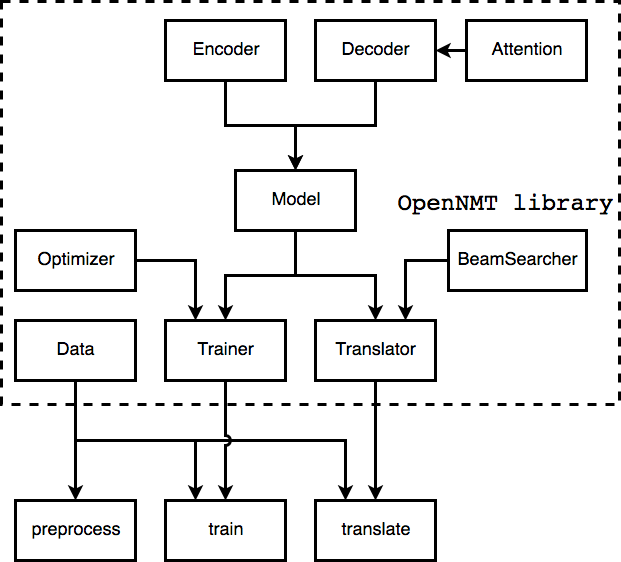
\includegraphics[scale=0.36]{OpenNMTDiagram.png}
        \caption{\label{fig:codestruct}Schematic overview of OpenNMT code}
        %\label{fig:opennmt-data}
    \end{figure}
A secondary goal was a desire for code readability and extensibility.
We targeted this goal by explicitly separating training, optimization and different components of the model, and by including tutorial documentation within
the code. A schematic overview of our data structures is shown in Figure~\ref{fig:codestruct}. We provide users with simple interfaces \textit{preprocess}, \textit{train} and \textit{translate}, which only require source/target files as input, while we provide a highly modularized library for advanced users. Each module in the library is highly customizable and configurable with multiple ready-for-use features, and we strive to update OpenNMT to reflect the latest research advances in the field.

\paragraph{Data Types} In addition to plain text, OpenNMT also supports input with discrete features \citep{sennrich2016linguistic}, as well as non-textual data such as image and speech. 
\paragraph{Model Types} OpenNMT implements various model types. On the encoder side in addition to RNN we also support CNN \citep{gehring2017convolutional}, Transformer \citep{vaswani2017attention}, image encoder \citep{DBLP:conf/conll/BowmanVVDJB16,DBLP:journals/corr/DengKR16} and audio encoder \citep{DBLP:journals/corr/ChanJLV15}. Likewise on the decoder side we also support CNN and Transformer. OpenNMT implements various attention types including general, dot product, and concatenation \citep{luong2015effective,britz2017massive}.
We also implemented copy mechanism \citep{vinyals2015pointer,gu2016incorporating}, which is widely used in document summarization.
\paragraph{Translation Constraints} In addition to out-of-vocabulary (OOV) handling \citep{Luong2015b}, OpenNMT also allows beam search with various normalizations including length and attention coverage normalization \citep{wu2016google}. We also provide interface for customized hypothesis filtering, enabling beam search under various constraints such as maximum number of OOV's and lexical constraints.


Due to the deliberate modularity of our code, OpenNMT is readily extensible for novel feature development. As one example, by substituting the attention module, we can arrive at local attention \citep{Luong2015}, sparse-max attention
\citep{martins2016softmax}, hierarchical attention \citep{yang2016hierarchical} and structured attention \citep{kim2017structured} with minimal change of code. As another example, in order to get feature-based factored neural translation \citep{sennrich2016linguistic} we simply need to modify the input network to process the feature-based representation, and the output network to produce multiple conditionally independent predictions. In addition to those thought experiments, in the real world, there are quite a few research groups using OpenNMT \citep{peters2017massively, levin2017toward, ha2017effective, sharaf2017umd, ameur2017arabic, sekizawa2017improving, ling2017coarse, ma2017osu, alvarez2017causal, van2017neural, gardent2017webnlg}, to name a few.


\subsection{Additional Tools}

OpenNMT provides many additional tools that make it more beneficial to the research community. A list of additional tools include: 1) reversible tokenizer, which can also perform Byte Pair Encoding (BPE) \citep{DBLP:journals/corr/SennrichHB15}; 2) loading and exporting word embeddings; 3) translation server which enables showcase results remotely; and 4) visualization tools for debugging or understanding, such as beam search visualization, profiler and TensorBoard/Crayon logging.


\begin{table}
\centering
          \begin{tabular}{l r}
          \toprule
            { System} & { BLEU-cased} \\
            \midrule
            uedin-nmt-ensemble & 28.3 \\
            LMU-nmt-reranked-wmt17-en-de & 27.1 \\
            {\bf SYSTRAN-single} & {\bf 26.7} \\
            \bottomrule
          \end{tabular}
          \caption{\label{tab:wmt}Top 3 on English-German \emph{newstest2017}.}
\end{table}



\begin{table}
  \centering
  \begin{tabular}{ccccc}
    \toprule
    Vocab & System & \multicolumn{2}{c}{Speed tok/sec}  & BLEU\\
     &  & Train  & Trans  &  \\
    \midrule
 V=50k & Nematus  & 3393 & 284 & 17.28 \\
     & ONMT  &4185 & 380 & 17.60 \\ 
    \midrule 
  V=32k & Nematus & 3221& 252 & 18.25 \\
    & ONMT &5254 & 457 & 19.34\\ 
    \bottomrule
  \end{tabular}

  \caption{ \small \label{tab:res} Performance Results for EN$\rightarrow$DE on WMT15 tested on \textit{newstest2014}. Both system 2x500 RNN, embedding size 300, 13 epochs, batch size 64, beam size 5. We compare on a 50k vocabulary and a 32k BPE setting.}
\end{table}

\section{Benchmarks}

OpenNMT achieves competitive results against other systems, e.g. in the recent WMT 2017 translation task, we got the third place in English-German translation with a single model as shown in Table~\ref{tab:wmt}. We expect performance and
memory usage to improve with further development.  Public benchmarks
are available at \url{http://opennmt.net/Models/}, which also includes
publicly available pre-trained models for all of these tasks and
tutorial instructions for all of these tasks. The benchmarks are
run on a Intel(R) Core(TM) i7-5930K CPU @ 3.50GHz, 256GB Mem,
trained on 1 GPU GeForce GTX 1080 (Pascal) with CUDA v. 8.0 (driver
375.20) and cuDNN (v. 5005).

The comparison, shown in Table~\ref{tab:res}, is on English-to-German
(EN$\rightarrow$DE) using the WMT
2015\footnote{\url{http://statmt.org/wmt15}} dataset. Here we compare,
BLEU score, as well as training and test speed to the publicly
available \textit{Nematus} system. 
\footnote{\url{https://github.com/rsennrich/nematus}. Comparison with
  OpenNMT/Nematus github revisions {\tt 907824}/{\tt 75c6ab1}.}


Additionally we have found interest from the community in using
OpenNMT for non-standard MT tasks like sentence document summarization and
dialogue response generation (chatbots), among others.  Using
OpenNMT, we were able to replicate the sentence summarization results
of \citet{chopra2016abstractive}, reaching a ROUGE-1 score of 33.13 on
the Gigaword data. We have also trained a model on 14 million
sentences of the OpenSubtitles data set based on the work
\citet{vinyals2015neural}, achieving comparable perplexity.


% which is remarkable since the corpus is completely parallel for
% the 5 languages which means that for a given language pair, no
% additional source or target sentence is presented to the system in
% another language pair.






%     Vocab 50k&  &  & 17.6/\\
%     \midrule
% BPE 32k&                &  & \\




% Picture of demo application running 

\section{Conclusion}

We introduce \textit{OpenNMT}, a research toolkit for NMT that
prioritizes efficiency and modularity. We hope to further develop
OpenNMT to maintain strong MT results at the research frontier, 
providing a stable and framework for production use.
\newpage
\small

\bibliographystyle{apalike}
\bibliography{writeup}


\end{document}
